\addbibresource{reference.bib}

\chapter{Energetická kalibrace}\label{calib}
Tato kapitola pojednává o metodách pro energetickou kalibraci hybridních částicových pixelových detektorů, pracujících v Time-Over-Treshold módu a o implementaci jedné z nich pro účely kalibrace detektorů sítě ATLAS TPX.

%********************************************************************************
% Motivace
%********************************************************************************
\section{Motivace}
Hybridní částicové pixelové detektory typu Timepix (viz \ref{det:tim}), disponují módem TOT (Time-Over-Treshold), který lze využít pro měření energie. Jak již bylo uvedeno v kapitole \ref{det:mod}, když částice interaguje s pixelem, pracujícím v tomto módu, ve kterém zanechá část své energie, dojde k vygenerování napěťového pulzu. Když je velikost tohoto pulzu větší, než treshold zasaženého pixelu, tak dojde je spuštění čítače, který začne počítat hodinové cykly měřící frekvence a zastaví se tehdy, když klesne hodnota napětí nazpět, pod úroveň tresholdu. Po skončení akvizice je hodnota tohoto čítače rovna hodnotě TOT, která zhruba odpovídá deponované energii interagující částice. Vztah mezi TOT a energií je ale silně nelineární a je podmíněn různými elektronickými a fyzikálními vlastnostmi daného pixelu. Určení tohoto vztahu je předmětem kalibrace, o které tato kapitola bude pojednávat.

%********************************************************************************
% Přehled kalibračních metod
%********************************************************************************
\section{Přehled kalibračních metod}

%********************************************************************************
% Přehled kalibračních metod
% > X-ray
%********************************************************************************
\subsection{Kalibrace detektorů za použití rentgenového záření}\label{calib:xray}
Metoda kalibrace pixelových detektorů pracujících v TOT módu \cite{Jakubek2011S262} spočívá v měření rentgenové fluorescence (viz \cite{Jakubek-radiography_and_charge_sharing}),
což je děj ke kterému dochází, když je nějaký materiál 
\footnote{Pro kalibraci se používají kovy, na příklad Am, In, Cu, Fe apod.}
ozařován rentgenovým zářením, které vyráží excitované elektrony z jeho atomů. Je-li vyražen elektron na nižší energetické úrovní, tak elektron z vyšší energetické úrovně deexcituje a obsadí jeho místo. Přebytečnou energii ztratí ve formě vyzářeného fotonu, který je následně detektorem detekován. 

Díky této fluorescenci je detektor pomocí různých mono-energetických zdrojů záření, jejichž energie je předem známa, postupně ozařován. V rámci tohoto měření je třeba pro každý zdroj pořídit velké množství snímků, ze kterých jsou následně vyfiltrovány jen tzv. \texttt{Single-Hit} události, což jsou události, při kterých interagující částice zasáhla jen jeden pixel. Tyto události jsou filtrovány z důvodu dosažení vyšší kvality kalibrace které je dosaženo potlačením zkreslení, způsobeným \texttt{Charge Sharing} efektem (viz \ref{det:mod}).

\begin{figure}[th]
	\begin{center}
		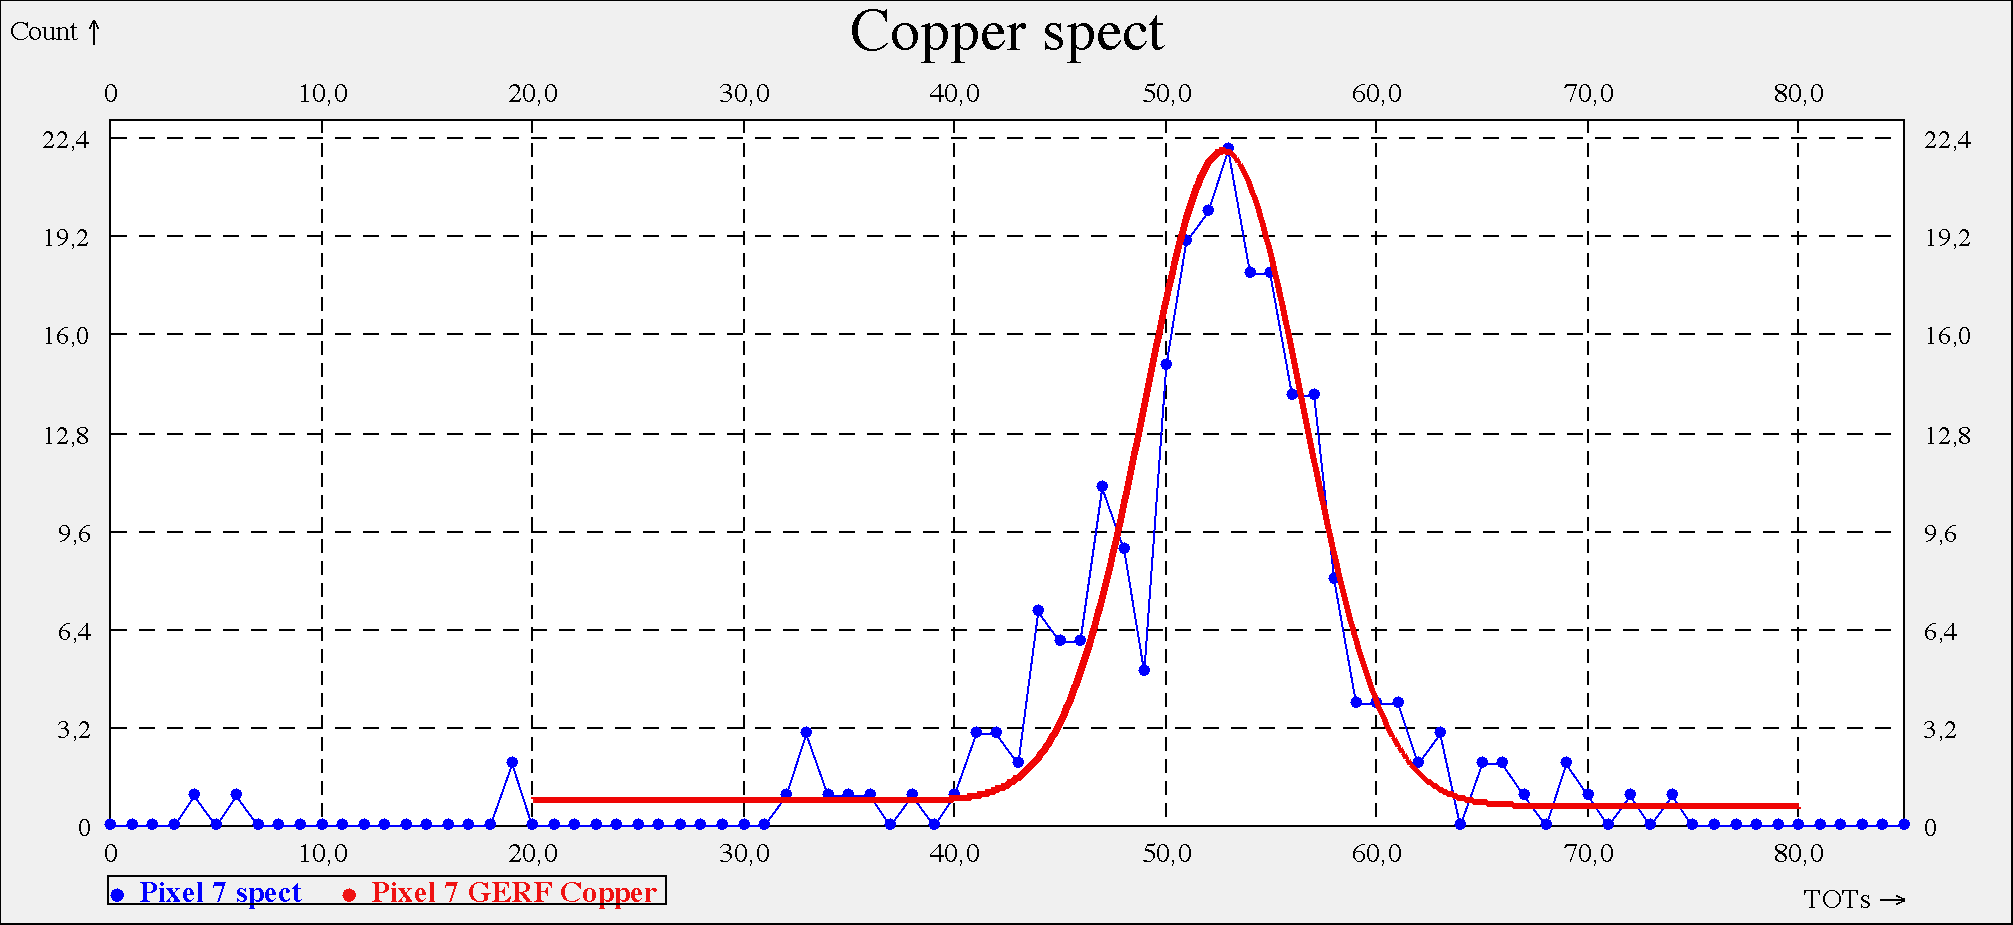
\includegraphics[width=14cm]{figures/calib_gerf.png}
		\caption{Spektrum TOT hodnot jednoho pixelu s proložením Gaussovou funkcí, sečtenou s Gaussovou chybovou funkcí (tzv. error funkce). Zdrojem rentgenové fluorescence byla měď.}
		\label{fig:calib:gerf}
	\end{center}
\end{figure}

Dalším krokem tohoto procesu je získání jednotlivých kalibračních bodů, udávající závislost mezi jednotlivými energiemi a TOT hodnotami. Toho je možné docílit vytvořením spekter pro jednotlivé pixely a zdroje záření. Na obrázku \ref{fig:calib:gerf} je příklad takového spektra pro jeden pixel detektoru a fluorescenčního záření z mědi. Na vodorovné ose tohoto spektra se nachází jednotlivé TOT hodnoty a na svislé pak jejich četnost ve všech snímcích. Z obrázku je patrné, že nejčetnější hodnotou TOT je zhruba hodnota $53$, které odpovídá energii fotonu, vyraženého z mědi, což je $5,9~keV$. Hodnotu TOT je ale třeba znát přesně, toho je docíleno proložením spektra funkcí \ref{eq:calib:gerf}, která vznikla z Gaussovy funkce, ke které z důvodu levé nesymetrie kvůli \texttt{Charge Sahring} efektu byla přičtena Gaussova chybová funkce. 

\begin{equation}\label{eq:calib:gerf}
	f_{GERF}(x) = \underbrace{Ae^{ -\frac{(x-\mu)^2}{2\sigma^2} }}_{\text{Gaussova funkce}} +
	\underbrace{ \frac{avg_{right} - avg_{left}}{\sigma\sqrt{2\pi}} \int_{-\infty}^t e^{ -\frac{(t-\mu)^2}{2\sigma^2} } + avg_{left}}_{\text{Gaussova chybová funkce}}
\end{equation}

Parametry funkce \ref{eq:calib:gerf} jsou následující:
\begin{itemize}
	\item $\mathbf{A}$ je amplituda.
	\item $\mathbf{\mu}$ je stření hodnota energie, kterou hledáme.
	\item $\mathbf{\sigma}$ udává rozptyl střední hodnoty energie a je možné ji vypočítat ze vzorce 
		$\sigma = \frac{2\sqrt{2ln_2}}{FWHM}$, kde $FWHM$\footnote{z angl. Full Width at Half Maximum} udává šířku gausiánu v polovině jeho výšky.
	\item $\mathbf{avg_{right}}$ (resp. $\mathbf{avg_{left}}$) je průměrná hodnoty spektra na pravém (resp. levém) úpatí gausiánu.
\end{itemize}
 
\begin{figure}[th]
	\begin{center}
		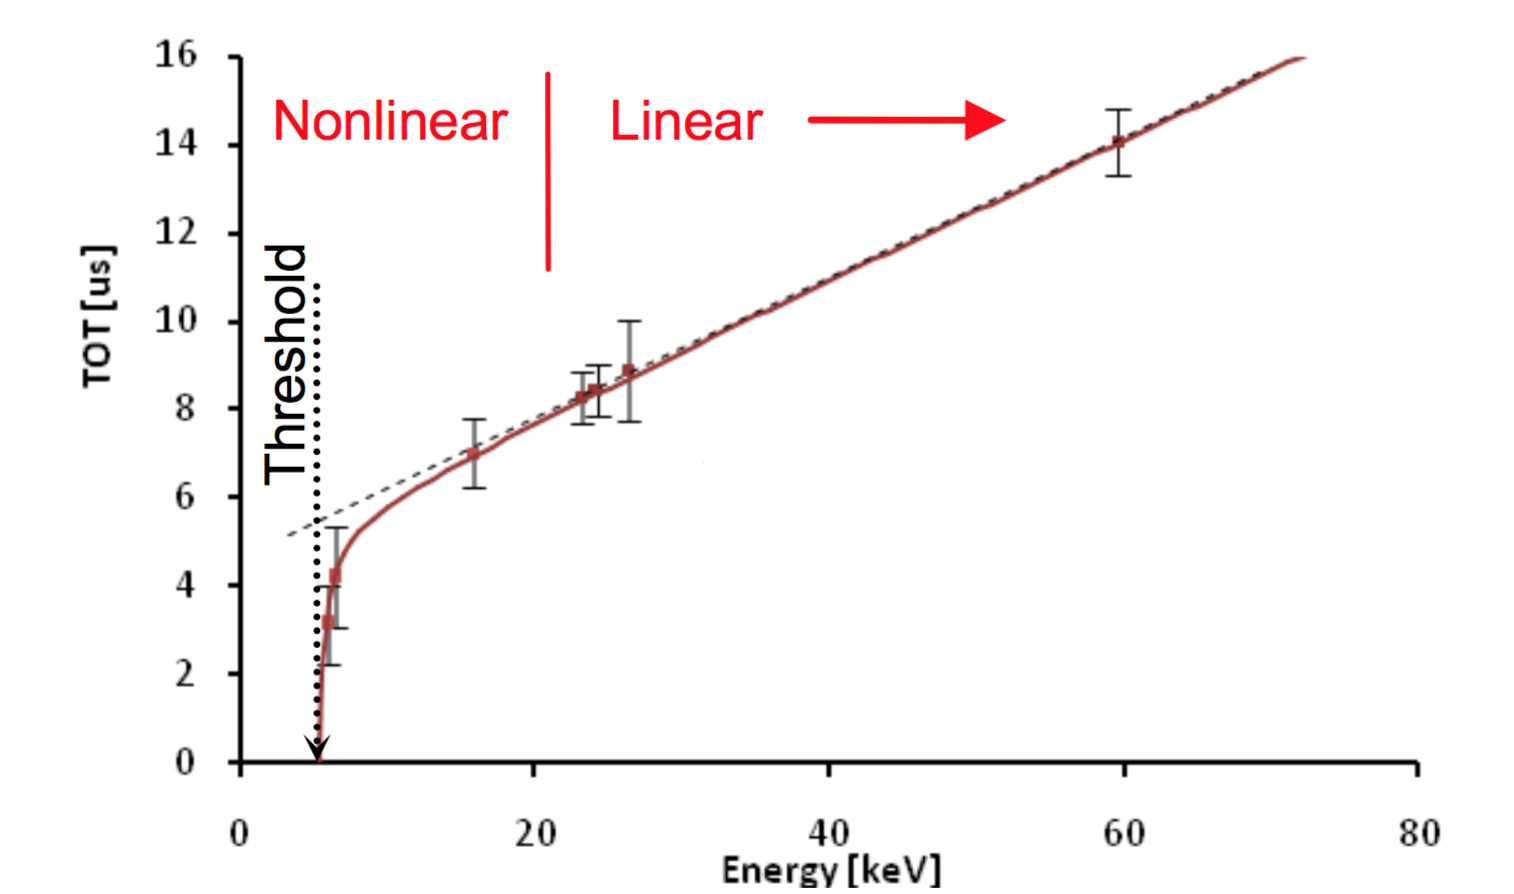
\includegraphics[width=13cm]{figures/calib_function.png}
		\caption{Kalibrační funkce (převzato z \cite{Jakubek2011S262})}
		\label{fig:calib:calib_function}
	\end{center}
\end{figure}

Z těchto kalibračních bodů je možné sestavit kalibrační funkci (viz vzorec \ref{eq:calib:calib_function}), udávající závislost mezi energií a TOT. Tato funkce vznikla složením hyperboly (popisující nelineární oblast nižších energií) a přímky (pro oblast s vyšší energií). Na obrázku \ref{fig:calib:calib_function} je znázorněn příklad této funkce.

\begin{equation}\label{eq:calib:calib_function}
	f_{calib}(x) = ax + b - \frac{c}{x-t}
\end{equation}


%********************************************************************************
% Přehled kalibračních metod
% > LED
%********************************************************************************
\subsection{Kalibrace detektorů pomocí LED diod}\label{calib:led}
Princip kalibrace pixelových detektorů (pracujících v TOT módu) pomocí SMD LED diod spočívá v působení přesného množství světelného záření na polovodičový senzor detektoru. V současné době je tato metoda ve fázi vývoje a doposud nebyla publikována. Metoda je použitelná pouze pro detektory, na jejímž senzoru není napařena tenká vrstva hliníku, která světelné záření nepropouští. 

Jako zdroj světla byl v ÚTEF ČVUT v Praze vyvinut modul s maticí $8\times8$ LED diod, který je možné ovládat pomocí \texttt{RS232} sériové linky. K tomuto modulu byl rovněž vyvinut plugin do softwarového balíku Pixelman \ref{det:pixelman}, který automatizuje proces nabírání dat této metody. Přes sériovou linku je schopen řídit modul s LED diodami a zároveň pomocí jádra Pixelmanu ovládá akvizici dat detektoru.

Kroky algoritmu této kalibrace jsou následující:
\begin{enumerate}
	\item Inicializace - nastavení spouštění akvizice detektoru na externí hardwarový trigger (který bude ovládán modulem s LED diodami), nastavení energie světelného záření (počet zabliknutí diody, délka periody jednoho bliknutí a doba aktivace diody v jedné periodě) a také délku akvizice snímku (vypočtené dle periody blikání a počet opakování).
	\item Měřící smyčka (opakuje se pro všechny LED diody). V rámci jednoho průchodu se provede následující:
		\begin{itemize}
			\item Zamaskování všech pixelů detektoru, krom těch pixelů, které jsou pod aktivní diodou.
			\item Spuštění akvizice.
			\item Vyčtení a uložení snímku z detektoru.
		\end{itemize}
	\item Následně se hodnoty všech snímků sečtou do jednoho snímku - viz obr. \ref{fig:calib:led_frame}.
\end{enumerate}

\begin{figure}[th]
	\begin{center}
		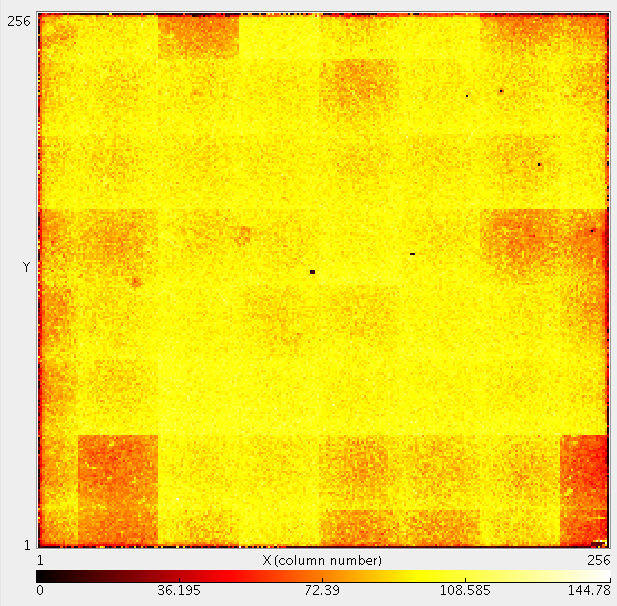
\includegraphics[width=10cm]{figures/led_calib_frame.png}
		\caption{Snímek z detektoru, ozařovaném modulem s LED diodami}
		\label{fig:calib:led_frame}
	\end{center}
\end{figure}

Z obrázku \ref{fig:calib:led_frame} jsou patrné hrany jednotlivých dílčích měření, které vznikly nehomogenitou elektronických vlastností jednotlivých diod. Tento jev může být odstraněn normalizací jejich světelné intenzity jejich kalibrací, jejíž výstupem bude kalibrační matice, kterou se vynásobí čas aktivace každé diody, což bude předmětem dalšího výzkumu této metody.

Tímto způsobem se pro každý pixel detektoru získají jednotlivé kalibrační body, které se následně proloží kalibrační funkcí (viz vzorec \ref{eq:calib:calib_function}), jak již bylo popsáno v kapitole \ref{calib:xray}.


%********************************************************************************
% X-ray Calib impl
%********************************************************************************
\section{Software pro kalibraci detektorů za použití rentgenového záření}

% osnova:
% proces kalibrace
% 	výběr vstupních dat
% 	analýza spekter (+ maska a tabulka)
% 	vytvoření kalibrační funkce (+ uložení dat, dodatečné úpravy calib fce, kvalita calib apod.)

% implementace

Tato podkapitola pojednává o softwaru pro energetickou kalibraci pixelových detektorů za použití kalibrační metody s rentgenovým zářením (viz \ref{calib:xray}). Tento software původně vznikal pro účely kalibrace sítě ATLAS TPX, avšak později byl rozšířen a nyní je kompatibilní se všemi detektory, pracující v TOT módu. Software vyl vyvinut v jazyce \texttt{Java} a grafické rozhraní bylo vytvořeno za pomoci knihovny \texttt{Swing}. V rámci této práce rovněž vznikla vlastní knihovna pro vizualizaci 2D grafů.

Jak již bylo zmíněno v kapitole \ref{calib:xray}, proces kalibrace se skládá z několika kroků, a to z vytvoření spekter pro jednotlivé pixely a zdroje záření, následném nalezení kalibračních bodů z těchto spekter a vytvoření kalibrační funkce pro každý pixel detektoru. Na obrázku \ref{fig:calib:sw_process_ops} je znázorněna možnost nastavení provedení jednotlivých kroků kalibračního procesu nad zvolenými měřeními (viz obr. \ref{fig:calib:sw_spektra} - levý postranní panel), v rámci jednoho průchodu po stisknutí tlačítka \texttt{Start/Abort} (viz obr. \ref{fig:calib:sw_spektra} vlevo dole).

\begin{figure}[th]
	\begin{center}
		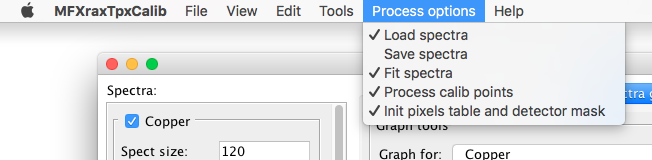
\includegraphics[width=14cm]{figures/calibsw_process_ops.png}
		\caption{Screenshot kalibračního softwaru - volby zpracování v rámci kalibračního procesu}
		\label{fig:calib:sw_process_ops}
	\end{center}
\end{figure}


%********************************************************************************
% X-ray Calib impl
% > Vstupní data kalibrace
%********************************************************************************
\subsection{Vstupní data kalibrace}
Vstupní data se skládají z několika měření pro různé zdroje fluorescenčního záření, jejichž energie jsou předem známy. Z těchto měření se vytvoří spektra pro každý pixel detektoru (příkladem takového spektra může být obrázek \ref{fig:calib:sw_spektra}, na kterém se screenshot kalibračního softwaru se spektrem jednoho pixelu pro měření fluorescence americia a india).

\begin{figure}[t]
	\begin{center}
		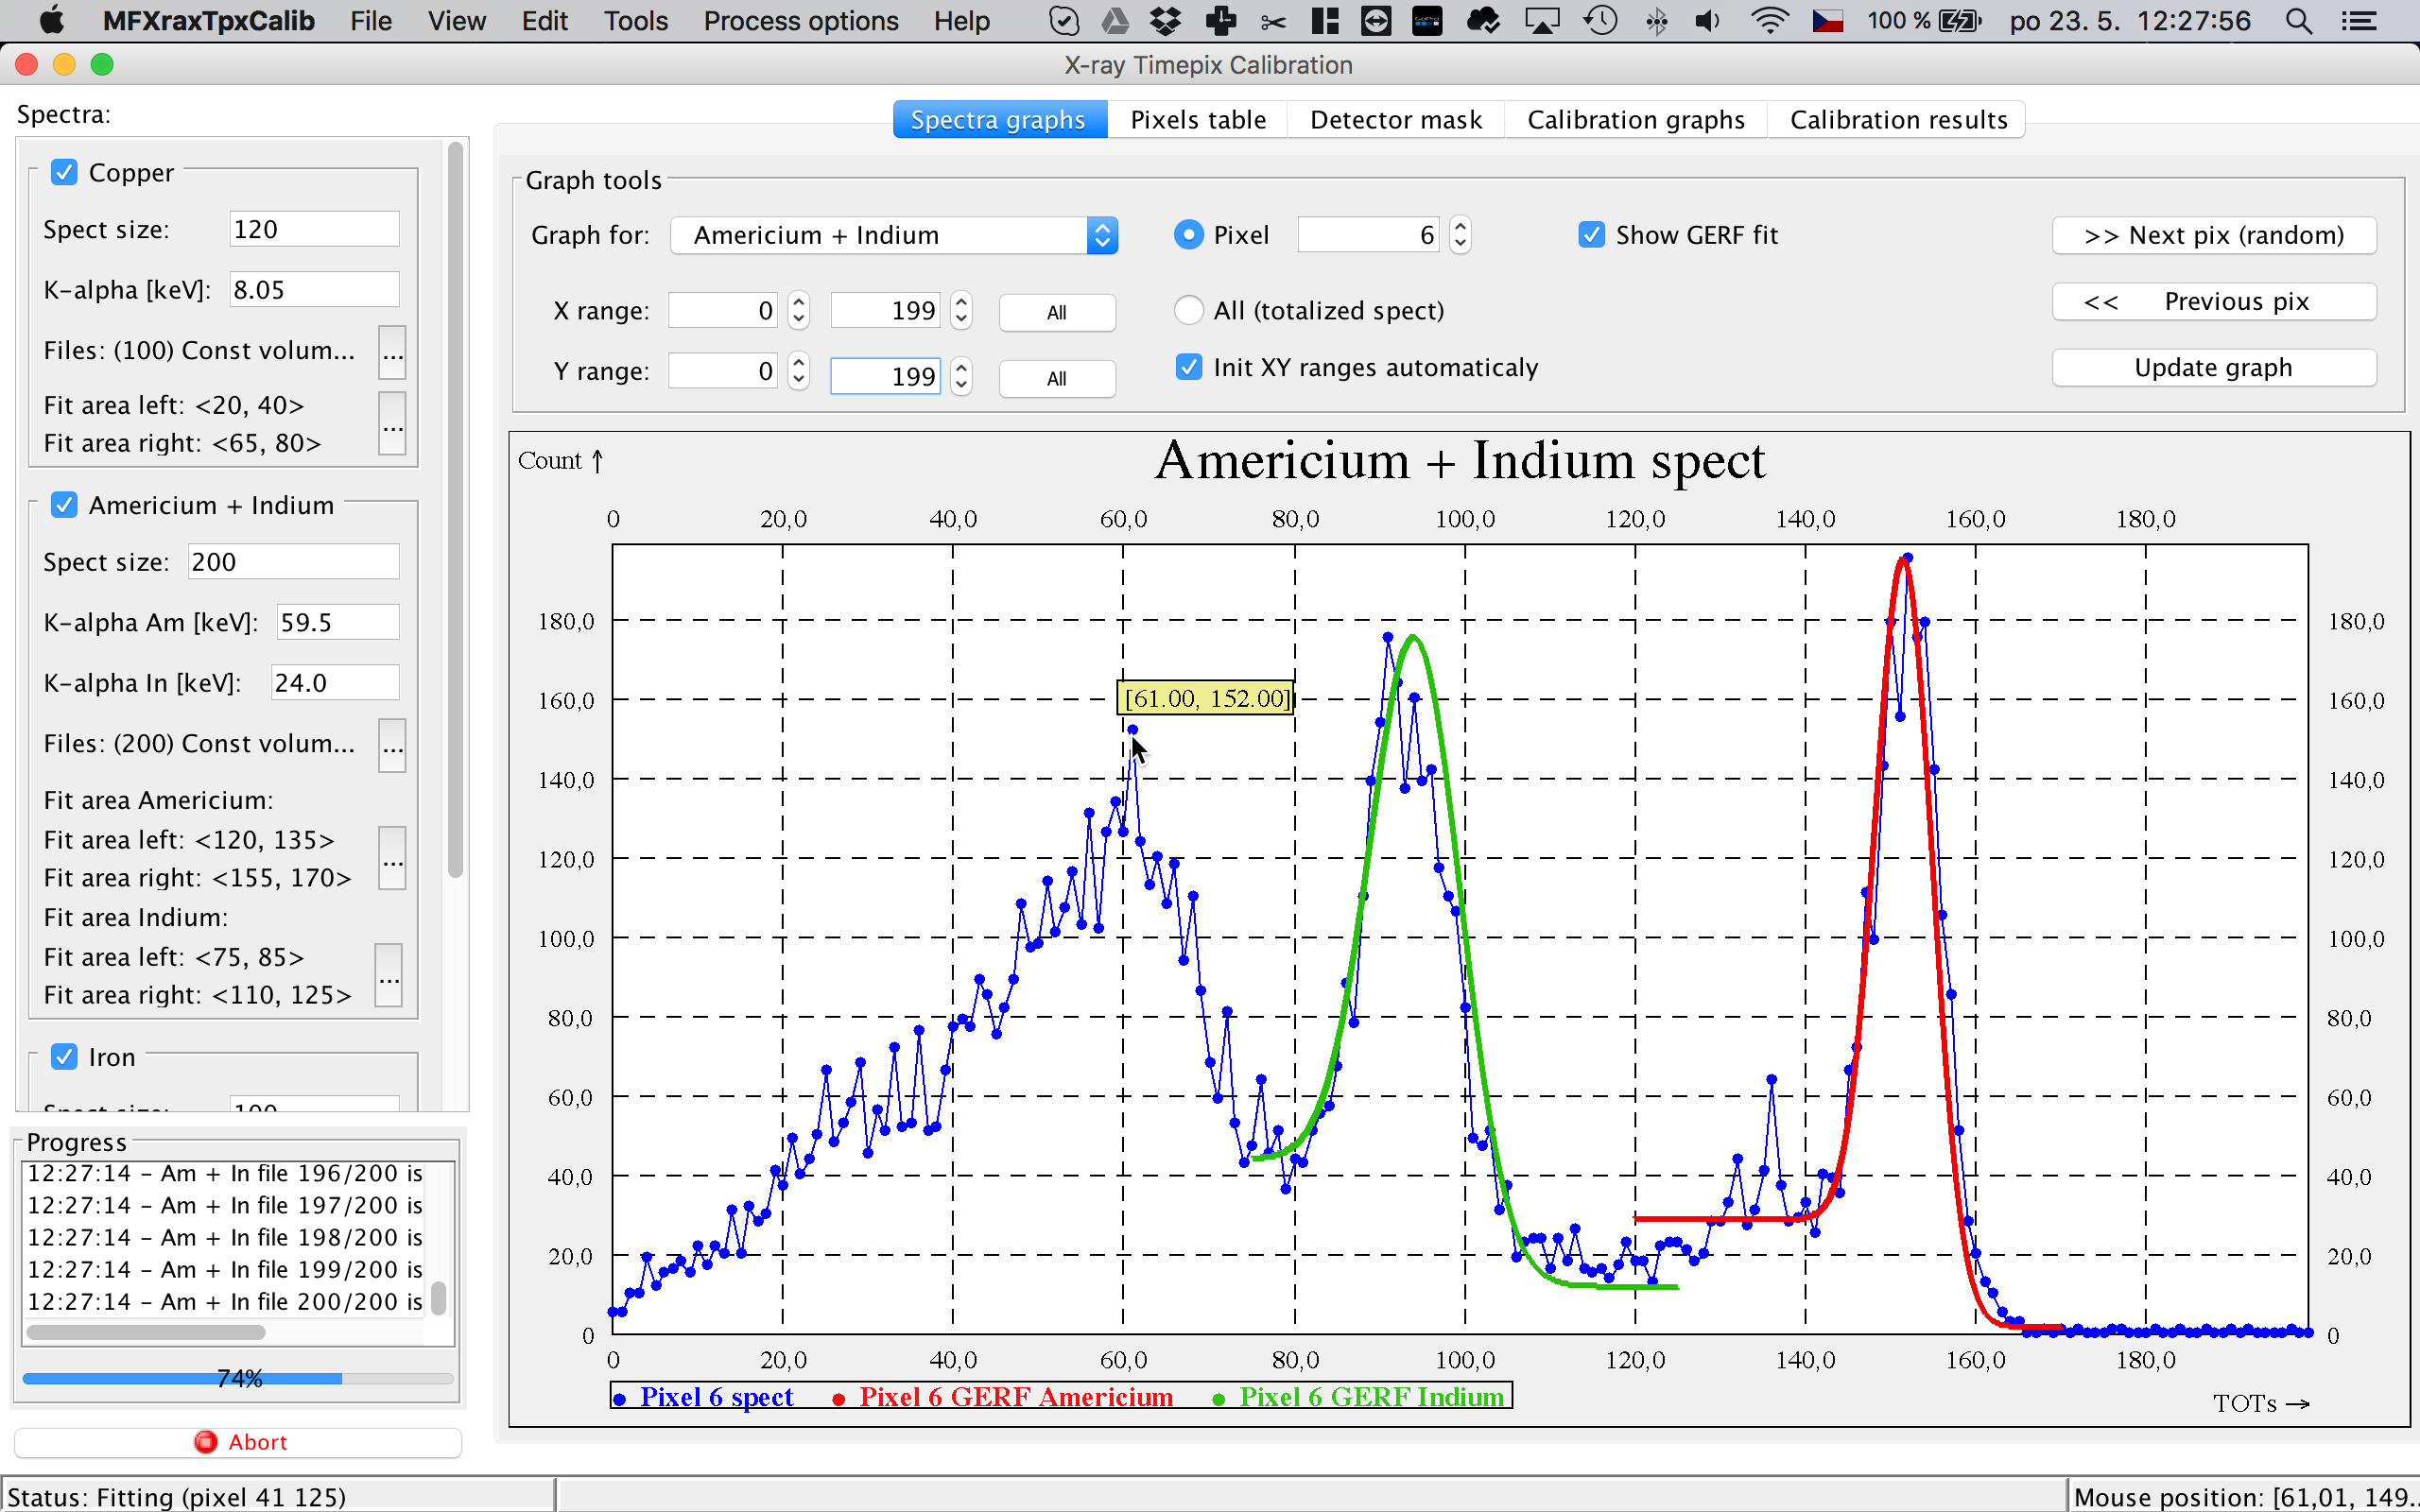
\includegraphics[width=15cm]{figures/calibsw_spectra_all.png}
		\caption{Screenshot kalibračního softwaru, zobrazující spektrum pro americium a indium, proložené funkcí \ref{eq:calib:gerf}}
		\label{fig:calib:sw_spektra}
	\end{center}
\end{figure}

K výběru vstupních dat slouží postranní panel hlavního okna kalibračního softwaru, kde je seznam jednotlivých měření. K manipulaci s položkami v tomto seznamu slouží \texttt{Measurement manager} (dostupný ze záložky \texttt{File} v hlavní liště - viz obr. \ref{fig:calib:sw_measurmanag}). V rámci tohoto nástroje je možné přidávat, odebírat, či jinak upravovat jednotlivá měření a jejich parametry (příklad velikost spektra apod.). Každé měření může obsahovat až tři kalibrační body (resp. zdroje fluorescenčního záření), jejichž parametry je možné také nastavit skrze \texttt{Measurement manager}.

\begin{figure}[th!]
	\begin{center}
		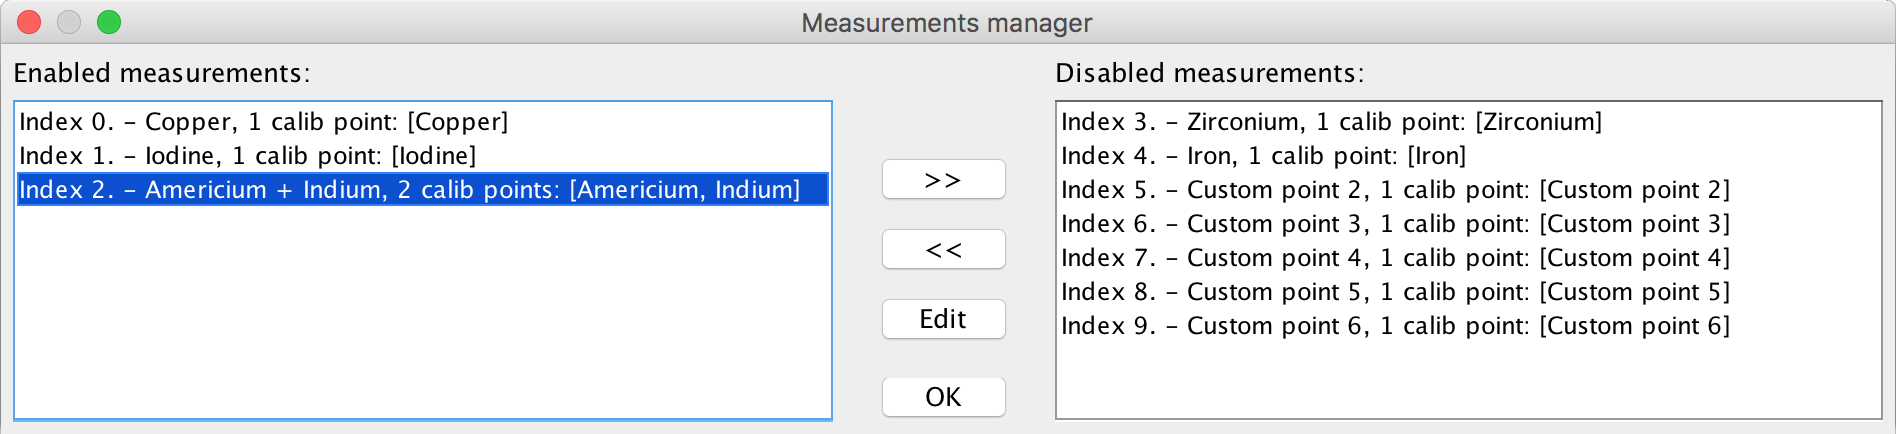
\includegraphics[width=15cm]{figures/calibsw_manager.png}
		\caption{Screenshot kalibračního softwaru - Measurement manager}
		\label{fig:calib:sw_measurmanag}
	\end{center}
\end{figure}

Vstupní data jsou podporována ve třech formátech:
\begin{description}
	\item[Multiframe] Multiframe formát slouží pro hromadné ukládání surových snímků z detektoru, kde jsou jednotlivé snímky zapsány jako seznam zasažených pixelů a jejich hodnot (pro více o tomto formátu viz \ref{atlas:cont:output}). Každý snímek je třeba načíst, vyfiltrovat pouze \texttt{Single-Hit} události (viz \ref{calib:xray}), ze kterých jsou následně vytvořena spektra pro všechny pixely.
	\item[Cluster log] Tento formát obsahuje snímky zapsané jako množinu clusterů, resp. shluků vzájemně sousedících pixelů s nenulovou hodnotou. Z těchto clusterů jsou vybrány jen clustery o velikosti jednoho pixelu (\texttt{Single-Hit} události), z kterých jsou následně vytvořena spektra.
	\item[Spektra] Tento formát obsahuje již zpracovaná spektra. Pro spektrum o velikosti $n$ hodnot jsou vstupní data tvořena $n$ soubory, kde každý soubor obsahuje matici výskytů $n$-té hodnoty spektra ve všech pixelech detektoru. Tento formát je nejvýhodnější, z důvodu malého objemu dat a zvýšení rychlosti zpracovávání dat (odpadá filtrování \texttt{Single-Hit} událostí).
\end{description}


%********************************************************************************
% X-ray Calib impl
% > Analýza spekter + maska + tabulka
%********************************************************************************
\subsection{Analýza spekter}\label{calib:sw:spektra}
Máme-li načtená vstupní data a z nich vytvořená spektra pro jednotlivé pixely detektoru a jednotlivá měření, je třeba v těchto spektrech nalézt hodnoty TOT, která odpovídá energii zdroje ionizujícího záření, použitém v daném měření. K tomu dochází pomocí proložení spekter funkce \ref{eq:calib:gerf} (viz \ref{calib:xray}). 

Tento algoritmus je v softwaru implementován za použití metody nejmenších čtverců. Úkolem tohoto algoritmu je nalézt takové parametry $A,~\mu,~\sigma,~avg_{left}~\text{a}~avg_{right}$ funkce \ref{eq:calib:gerf} tak, aby hodnota funkce \ref{eq:sq:rms} byla minimální, resp. aby suma čtverců vzdáleností jednotlivých hodnot spektra a jejich příslušných funkčních hodnot funkce \ref{eq:calib:gerf} (tzv. reziduí) byla minimální.

\begin{equation}\label{eq:sq:rms}
	E = \frac{1}{N} \sum_{i=0}^{N}(f_{GERF}(i) - count_i)^2
\end{equation}

Jedná se o iterativní metodu, kde hodnota jednotlivé parametry $A,~\mu,~\sigma,~avg_{left}~\text{a}~avg_{right}$ jsou v rámci jednotlivých iterací postupně vylepšovány, resp. hodnota funkce \ref{eq:sq:rms} je minimalizována. Jelikož všechny tyto parametry jsou na sobě nezávislé, v rámci jedné iterace optimum každého z parametrů může být získáno pomocí Gradientní metody.

Algoritmus této metody je následující: Nejprve se k danému parametru přičte konstanta základního kroku a sleduje se změna sumy reziduí. Když se tato suma zvětší, jedná se o znamení špatného směru kroku, který je třeba vrátit a konstantu základního kroku násobit~$-1$. Dále se vy smyčce přičítá postupně se zvětšující násobek základního kroku a sleduje se změna sumy reziduí. Začne-li se tato suma zvětšovat, vrátí se aktuální krok zpátky a algoritmus končí. Toto se v rámci jedné iterace provede pro všechny zkoumané parametry.

Počet těchto iterací je možné v softwaru nastavit v hlavní liště (\texttt{Edit > Set number of iterations}), jelikož tato metoda konverguje relativně rychle, optimální (z hlediska doby a kvality kalibrace) počet iterací je 3-5.

Z nalezených optimálních parametrů $A,~\sigma,~avg_{left}~\text{a}~avg_{right}$, resp. z odchylky od jejich mediánu je možné pro každý pixel určil jeho kvalitu, jejímž výstupem maska špatných pixelů detektoru. Na obrázku \ref{fig:calib:sw_mask} je znázorněna vizualizace této masky. Maska může být generována na základě jednoho z parametrů, nebo všech parametrů dohromady a může byt uložena v textové podobě (matice hodnot, kde $0$ znamená nezamaskovaný a $1$ zamaskovaný pixel).

\begin{figure}[th!]
	\begin{center}
		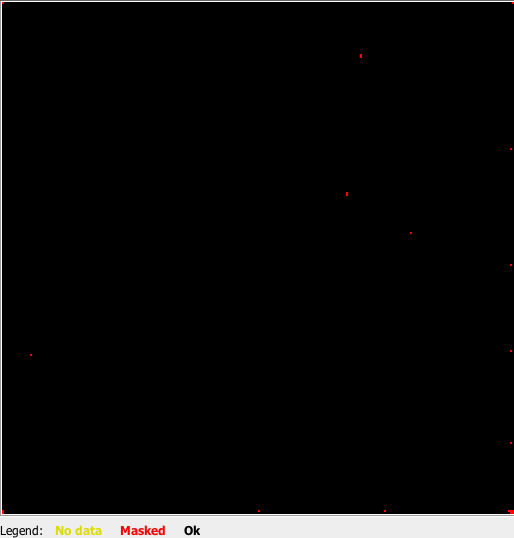
\includegraphics[width=10cm]{figures/calibsw_mask.png}
		\caption{Screenshot kalibračního softwaru - maska špatných pixelů}
		\label{fig:calib:sw_mask}
	\end{center}
\end{figure}


%********************************************************************************
% X-ray Calib impl
% > vytvoření kalibrační funkce (+ uložení dat, dodatečné úpravy calib fce, kvalita calib apod.)
%********************************************************************************
\subsection{Vytvoření kalibrační funkce}
Když jsou ze spekter získané jednotlivé kalibrační body, je možné přikročit k dalšímu kroku kalibračního procesu, a to vytvoření kalibrační funkce pro každý pixel detektoru (viz obr. \ref{fig:calib:sw_calib_function}). Tato úloha spočívá v položení kalibračních bodů jednotlivých pixelů kalibrační funkcí \ref{eq:calib:calib_function}, resp. nalezení takových parametrů $a~,b~,c~\text{a}~t$ kalibrační funkce \ref{eq:calib:calib_function} tak, aby součet reziduí byl minimální (viz \ref{calib:sw:spektra}).

\begin{figure}[t]
	\begin{center}
		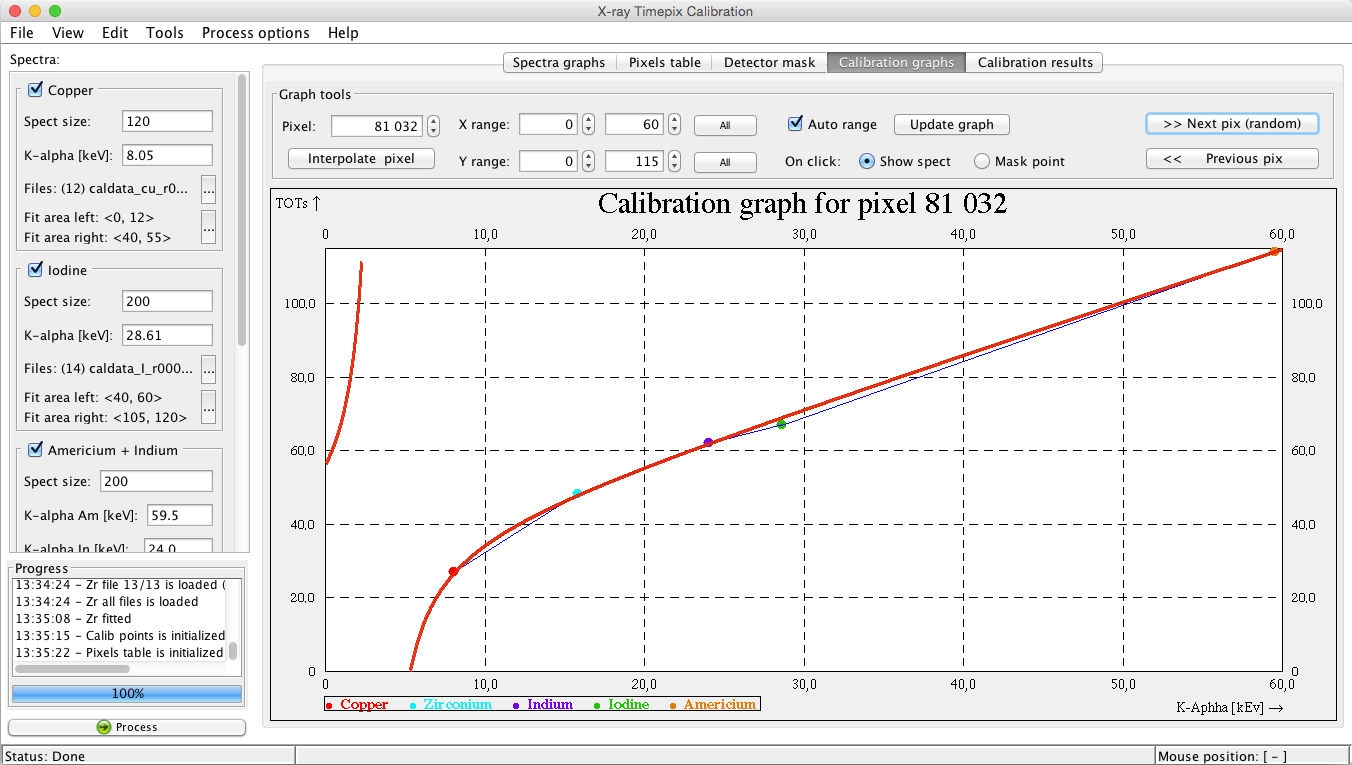
\includegraphics[width=15cm]{figures/calibsw_cc.png}
		\caption{Screenshot kalibračního softwaru - kalibrační funkce}
		\label{fig:calib:sw_calib_function}
	\end{center}
\end{figure}

Jednotlivé parametry kalibrační funkce \ref{eq:calib:calib_function} jsou vzájemně závislé, proto pro nalezení těchto parametrů nelze použít stejný algoritmus, jako při analýze spekter (\ref{calib:sw:spektra}). Tato metoda byla navržena tak, aby bylo schopná kalibrační funkci vytvořit ze dvou bodů. Počet kalibračních bodů je variabilní položkou, roto pro nalezení parametrů kalibrační funkce \ref{eq:calib:calib_function} jsou použity různé algoritmy.

\begin{description}
	\item[Algoritmus pro dva body]
	Při kalibraci pomocí dvou kalibračních bodů je uživatel vyzván k zadání parametru $c$ a $t$ kalibrační funkce. Zbylé parametry jsou vypočteny pomocí soustavy rovnic \ref{eq:calib:2points} a dvou známých kalibračních bodů.
	\begin{eqnarray}\label{eq:calib:2points}
		ax_{1} + b - \frac{c}{x_{1}-t} &=& y_{1} \\
		ax_{2} + b - \frac{c}{x_{2}-t} &=& y_{2} \nonumber 
	\end{eqnarray}
	Při parametrizování parametrů $c$ a $t$ vzniká velká nepřesnost, především v nelineární oblasti nižších energiích, proto tato metoda pro dva body je nejméně přesná.

	\item[Algoritmus pro tři body]
	Tří-bodová kalibrace je oproti dvou-bodové kalibraci značně přesnější. Nicméně protože kalibrační funkce má čtyři parametry, je třeba nějaký z nich parametrizovat. Proto uživatel na začátku kalibračního procesu bude vyzván k zadání parametru $t$ a zbylé parametry budou vypočteny ze soustavy rovnic \ref{eq:calib:3points}.
	\begin{eqnarray}\label{eq:calib:3points}
		ax_{1} + b - \frac{c}{x_{1}-t} &=& y_{1} \nonumber \\
		ax_{2} + b - \frac{c}{x_{2}-t} &=& y_{2} \\
		ax_{3} + b - \frac{c}{x_{3}-t} &=& y_{3}\nonumber 
	\end{eqnarray}

	\item[Algoritmus pro čtyři body]
	Algoritmus pro čtyři body je o něco komplikovanější. Nejprve parametr $t$ je parametrizován (bez zásahu uživatele). Poté parametry $a,~b~\text{a}~c$ jsou vypočteny pomocí třech bodů soustavy rovnic \ref{eq:calib:3points}. Tyto tři body jsou vybrány následovně:
	\begin{description}
		\item[1. bod] je vybrán jako bod s nejnižší energií.
		\item[2. bod] je vybrán z některého z prostředních bodů (ve výchozím nastavení 2. bod s nejnižší energií - možné změnit v \texttt{Edit > Adjust middle trial point}).
		\item[3. bod] je vybrán jako bod s nejvyšší energií.
	\end{description}

	Poté pomocí metody bisekce a metody nejmenších čtverců je nalezena taková hodnota parametru $t$, že jeho reziduum je minimální, v ideálním případě nulové.

	\item[Algoritmus pro pět a více bodů]
	První část algoritmu pro pět a více bodů se od algoritmu pro čtyři body nikterak neliší - pomocí třech bodů (volba prostředního je opět na uživateli) jsou vypočteny parametry $a,~b~\text{a}~c$ a poté pomocí metody bisekce a čtvrtého bodu je určen parametr $t$. V ideálním případě prochází funkce \ref{eq:calib:calib_function} všemi čtyřmi body, nebo alespoň jejich rezidua jsou minimální. 

	Nyní je třeba ještě zohlednit pátý bod (po př. další body). Tomu se děje pomocí metody bisekce a metody nejmenších čtverců, přičemž v rámci jedné iterace tohoto algoritmu se mění všechny parametry (jelikož jsou vzájemně závislé). Postupně se ke každému parametru přičte konstanta základního kroku a sleduje se změna sumy residuí. Z těchto změn se vytvoří vektor směru změny všech parametrů. Pomocí metody bisekce se násobek tohoto vektoru v jednotlivých krocích k parametrům funkce přičítá, přičemž se sleduje změna sumy reziduí. Daná iterace končí, když suma reziduí se přestane zmenšovat.

	Počet těchto iterací uživatel může opět nastavit hlavní liště (\texttt{Edit > Set number of iterations}).

\end{description}

Po dokončení procesu kalibrace software nabízí v záložce \texttt{Calibration graphs} zobrazení kalibrační funkce pro jednotlivé pixely detektoru. Na tomto místě je možné jednotlivé pixely interpolovat (více v \ref{calib:sw:post_process}), nebo kliknutím na daný kalibrační bod je možné dle preferencí uživatele ho buď zamaskovat, nebo zobrazit jeho spektrum. Software rovněž umožňuje hromadné maskování kalibračních bodů ve zvoleném intervalu (\texttt{Tools > Batch calib points masking} v hlavní liště).

Výstupní data tvoří $a~,b~,c~\text{a}~t$ parametry kalibrační funkce \ref{eq:calib:calib_function}, které je možné uložit pomocí \texttt{File > Save calib files} v hlavní liště. Tato data je možné uložit v samostatných souborech pro každý parametr, kde hodnoty daného parametru pro jednotlivé pixely jsou zapsány v matici, nebo je možné tato data uložit do jednoho souboru, kde jednotlivé parametry jsou zapsány ve sloupcích.


%********************************************************************************
% X-ray Calib impl
% > Dodatečné úpravy
%********************************************************************************
\subsection{Dodatečné úpravy}\label{calib:sw:post_process}
Tento kalibrační software rovněž nabízí i nástroje pro vizualizaci kvality kalibrace. K tomuto účelu slouží záložka \texttt{Calibration results}, kde v rámci bočního pohledu na detektor je možné si v grafu zobrazit všechny hodnoty vybraného parametru kalibrační funkce \ref{eq:calib:calib_function} - viz obr. \ref{fig:calib:sw_calib_results}.

Díky této vizualizaci výsledků kalibrace je možné snadno odhalit případnou deviaci některého z parametrů pro určitý pixel detektoru. Kalibrační hodnoty pro takto poškozený pixel je možné upravit - na příklad pomocí interpolace hodnot čtyřech sousedních pixelů (spojených hranou s daným pixelem). Pixely je možné interpolovat samostatně, nebo automaticky pomocí nástroje zvaném \texttt{Batch interpolating} (v záložce \texttt{Tools} lavní lišty), který uživateli umožňuje zvolit rozsah hodnot daného parametru, ve kterém budou všechny pixely interpolovány.

\begin{figure}[t]
	\begin{center}
		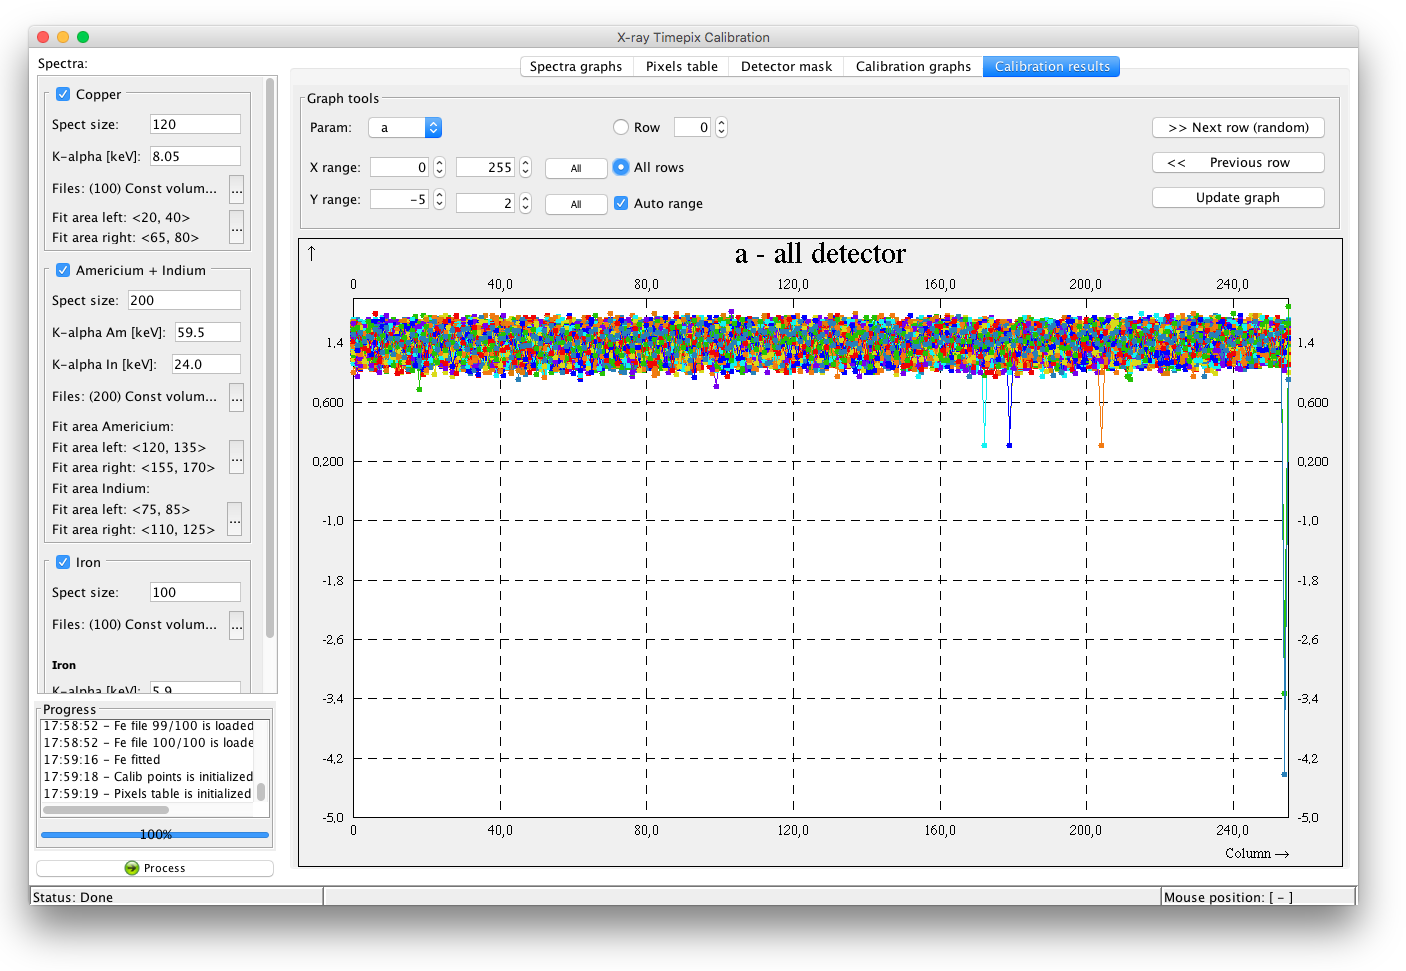
\includegraphics[width=16cm]{figures/calibsw_result.png}
		\caption{Screenshot kalibračního softwaru - vizualizace výsledných parametrů kalibrace}
		\label{fig:calib:sw_calib_results}
	\end{center}
\end{figure}









